\documentclass{minimal}
\usepackage{tikz}
\usetikzlibrary{automata,positioning}

\begin{document}
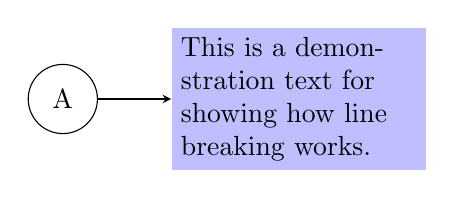
\begin{tikzpicture}[%
    >=stealth,
    node distance=3cm,
    on grid,
    auto
  ]
  \node[state] (A)              {A};
  \node        (B) [right of=A,fill=blue!25,text width=3cm]{This is a demonstration text for showing how line breaking works.};;
  \path[->] (A) edge (B);
\end{tikzpicture}
\end{document}







%% \documentclass{article}
%% \usepackage{tikz}
%% \usepackage{amsmath}
%% \begin{document}
%% \begin{tikzpicture}[every node/.style={rectangle,draw}]

%% \end{tikzpicture}
%% \end{document}
